\documentclass{article}
\usepackage[english]{babel}
\usepackage{amsfonts, amsmath, amssymb, MnSymbol, graphicx, algpseudocode, algorithm, amsthm}
\usepackage{hyperref}

\numberwithin{figure}{section}

%%% Helpers
\newcommand{\algtab}{\hspace{\algorithmicindent}}
\newcommand{\wi}{\omega_i}
\newcommand{\hsigma}{\widehat \Sigma}
\newcommand{\hmu}{\hat \mu}

%%% Shortcuts
\newcommand{\bx}{\mathbf{x}}
\newcommand{\bm}{\mathbf{\mu}}
\newcommand{\bsig}{\mathbf{\Sigma}}

%%% Draft helpers (remember to remove when done)
\newcommand{\outline}[2]{\paragraph{\textsc{#1}}\hrulefill~\\{\small\it #2}\\\_\hrulefill}
\newcommand{\todo}[1]{\outline{\large TODO}{#1}}

%%%%%%%%%%%%%%%%%%%%%%%%%%%%%%%%%%%%%%%%%%%%%%%%%%%%%%%%%%%%%%%%%%%%%%%%%%%%%%%%%%%

\title{CAP5638 Project 1\\
\large Classification Using Maximum-likelihood, Parzen Window, and $k$-Nearest Neighbors}
\author{Suhib Sam Kiswani}
\date{October 26, 2015}

%%%%%%%%%%%%%%%%%%%%%%%%%%%%%%%%%%%%%%%%%%%%%%%%%%%%%%%%%%%%%%%%%%%%%%%%%%%%%%%%%%%

\begin{document}
\maketitle

\begin{enumerate}
\item redo classification results using max leave one training point out success rates.
\end{enumerate}

The algorithms were implemented in {\it Python 3.4}, with a dependence on the \textit{scipy} \cite{sp} library.

%%%%%%%%%%%%%%%%%%%%%%%%%%%%%%%%%%%%%%%%%%%%%%%%%%%%%%%%%%%%%%%%%%%%%%%%%%%%%%%%%%%
\section{Maximum likelihood estimation}
\subsection{Parametric Forms}
%~~~~~~~~~~~~~~~~~~~~~~~~~~~~~~~~
\subsubsection{Normal Density}
The discriminant function for the normal density is:

$$g_i(\bx) = \bx^T\mathbf{W}_i\bx + \mathbf{w}_i^T \bx + w_{i0}$$
where:
$$\mathbf{W}_i = -0.5 \bsig_i^{-1}$$
$$\mathbf{w}_i = \bsig_i^{-1} \bm_i$$
$$w_{i0} = -0.5 \bm_i^T \bsig_i^{-1} \bm_i - 0.5\ln \left( \det \bsig_i \right) + \ln P(\omega_i)$$

Using the training samples, the mean and covariance can be estimated with maximum likelihood using the following definitions:
\begin{align*}
\hat\bm_i = \frac{1}{n} \sum^n_{k=1} \bx_k &~& \widehat\bsig_i = \frac{1}{n} \sum^n_{k=1} (\bx_k - \hat\bm_i)(\bx_k - \hat\bm_i)^T
\end{align*}

Which yields:
$$p(\bx|\mathbf{\omega_i}) = \frac{1}{\sqrt{(2 \pi)^n \det \widehat\bsig_i}} \exp\left( -\frac{1}{2} (\bx - \hat\bm_i)^T \widehat\bsig_i^{-1} (\bx - \hat\bm_i) \right)$$

The classification of instance $\bx$ is $\mathbf{\omega_i} = \arg\max_{\mathbf{\omega_i}} \left| p(\bx|\mathbf{\omega_i}) P(\mathbf{\omega_i}) \right|$

%~~~~~~~~~~~~~~~~~~~~~~~~~~~~~~~~
\subsubsection{Uniform}
\todo{write out eqns}

%%%%%%%%%%%%%%%%%%%%%%%%%%%%%%%%%%%%%%%%%%%%%%%%%%%%%%%%%%%%%%%%%%%%%%%%%%%%%%%%%%%
\subsection{Experimental Results}
\subsubsection{Iris Data Set}
\begin{enumerate}
\item {\bf Normal Density}
The estimated parameters of $\hat\theta$ for each of the classes from the training samples were:
$$\hat\bm_1 = \left( 4.98181818,  3.39090909,  1.45151515,  0.25151515 \right)$$
$$\widehat\bsig_1 = \begin{pmatrix}
    0.10876033 & 0.08619835 & 0.02033058 & 0.01093664\\
    0.08619835 & 0.13597796 & 0.01410468 & 0.00865014\\
    0.02033058 & 0.01410468 & 0.03401286 & 0.00825528\\
    0.01093664 & 0.00865014 & 0.00825528 & 0.0134068
\end{pmatrix}$$

$$\hat\bm_2 = \left( 5.89090909,  2.78787879,  4.26363636,  1.31515152 \right)$$
$$\widehat\bsig_2 = \begin{pmatrix}
    0.2353719  & 0.06867769 & 0.165427   & 0.05256198\\
    0.06867769 & 0.08530762 & 0.07743802 & 0.04442608\\
    0.165427   & 0.07743802 & 0.20110193 & 0.06933884\\
    0.05256198 & 0.04442608 & 0.06933884 & 0.0394674
\end{pmatrix}$$

$$\hat\bm_3 = \left( 6.66060606,  2.94848485,  5.58484848,  1.99393939 \right)$$
$$\widehat\bsig_3 = \begin{pmatrix}
    0.36359963 & 0.11887971 & 0.2851607  & 0.03976125\\
    0.11887971 & 0.10613407 & 0.08861341 & 0.03817264\\
    0.2851607  & 0.08861341 & 0.29219467 & 0.03202938\\
    0.03976125 & 0.03817264 & 0.03202938 & 0.06784206
\end{pmatrix}$$

\smallskip

This method correctly classified $48$ of the $51$ testing samples ($94.1$\% accuracy).
\todo{add decision boundary graphs}

\item {\bf Uniform}
\todo{gotta do it}
\end{enumerate}

\subsubsection{UCI Wine Data Set}

%%%%%%%%%%%%%%%%%%%%%%%%%%%%%%%%%%%%%%%%%%%%%%%%%%%%%%%%%%%%%%%%%%%%%%%%%%%%%%%%%%%
\section{Parzen window estimation}
The window function is:
$$\phi(\bx) = \left\{\begin{matrix}
1 & |\bx_j| \leq 1/2; & j \in [1,...,d]\\
0 & otherwise &
\end{matrix}\right.$$

with constants:
$$V_n = h_n^d$$

\begin{enumerate}
\item {\bf Hypercube Kernel}
$$p(\bx | \omega_i ) = \frac{1}{n} \sum^n_{i=1} \frac{1}{V_n} \phi \left(\frac{\bx - \bx_i}{h_n}\right)$$

\item {\bf Gaussian Kernel}
$$p(\bx | \omega_i ) = \frac{1}{n} \sum^n_{i=1} \frac{1}{V_n} \phi \left(\frac{1}{\sqrt{2\pi}^d V_n} \exp\left[-\frac{1}{2} \left(\frac{\bx - \bx_i}{h_n}\right)^2\right]\right)$$
\end{enumerate}

All data processed by this classifier was transformed using the \emph{z-score}:
$$\mathbf{z_x} = \frac{\bx - \bm}{\mathbf{\sigma}}$$

%%%%%%%%%%%%%%%%%%%%%%%%%%%%%%%%%%%%%%%%%%%%%%%%%%%%%%%%%%%%%%%%%%%%%%%%%%%%%%%%%%%
\subsection{Experimental Results}
For all given data sets, the \emph{Hypercube kernel} was the most accurate method.

\subsubsection{Iris Data Set}
\begin{figure}[H]
\centering
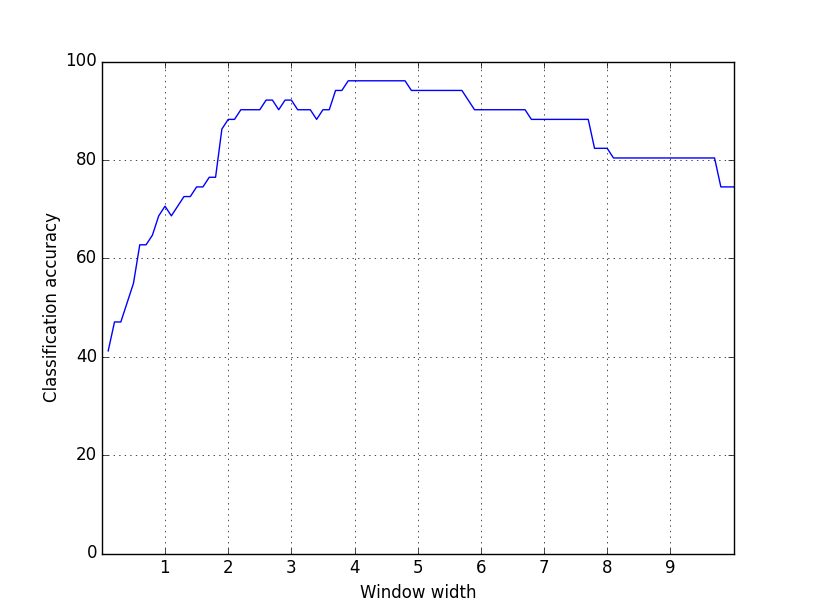
\includegraphics[width=.8\textwidth]{p_box_iris}
\caption{Accuracy of the Parzen window classifier using the \emph{Hypercube kernel} across different window widths for the iris data set.}
\label{pb_iris}
\end{figure}

\begin{figure}[H]
\centering
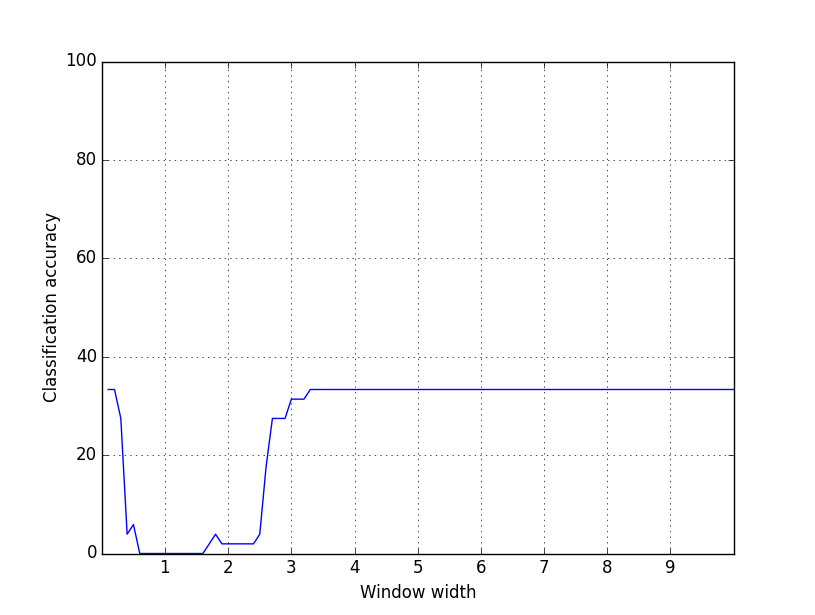
\includegraphics[width=.8\textwidth]{pg_iris}
\caption{Accuracy of the Parzen window classifier using the \emph{Gaussian kernel} across different window widths for the iris data set.}
\label{pg_iris}
\end{figure}

\subsubsection{UCI Wine Data Set}
\begin{figure}[H]
\centering
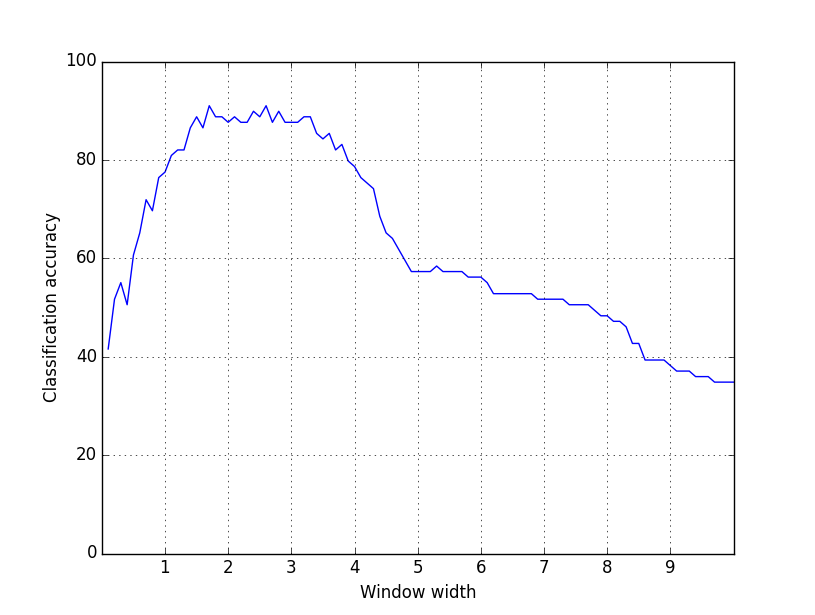
\includegraphics[width=.8\textwidth]{p_box_wine}
\caption{Accuracy of the Parzen window classifier using the hypercube window function across different window widths for the wine data set.}
\label{pb_wine}
\end{figure}

\begin{figure}[H]
\centering
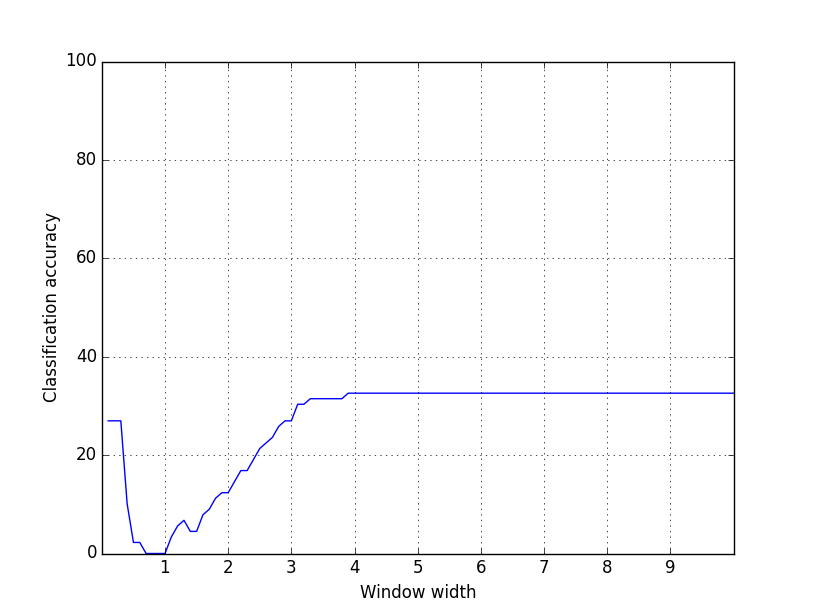
\includegraphics[width=.8\textwidth]{pg_wine}
\caption{Accuracy of the Parzen window classifier using the \emph{Gaussian kernel} across different window widths for the wine data set.}
\label{pg_wine}
\end{figure}


\subsubsection{Handwritten Digits Data Set}

%%%%%%%%%%%%%%%%%%%%%%%%%%%%%%%%%%%%%%%%%%%%%%%%%%%%%%%%%%%%%%%%%%%%%%%%%%%%%%%%%%%
\section{$k$-nearest neighbors}
The $k$-nearest neighbors classifier was implemented using a $kd$-tree, subdividing along the median of the training data. This distance metric $d$ used for this classifier was Euclidean distance ($||\bx - \textbf{y}||$).

\todo{{\bf Speed up using k-d tree} With k from 1 to 10 with an increment of 1, first build a k-d tree from the training set and then classify the test samples using the k-nearest neighbor classifier by finding the nearest neighbors using the k-d tree. Compare the classification accuracy and the number of distance calculations with the basic k nearest neighbor implementation on the three datasets. Summarize your observations and justify your results.}

%%%%%%%%%%%%%%%%%%%%%%%%%%%%%%%%%%%%%%%%%%%%%%%%%%%%%%%%%%%%%%%%%%%%%%%%%%%%%%%%%%%
\subsection{Experimental Results}
\subsubsection{Iris Data Set}
\begin{figure}[H]
\centering
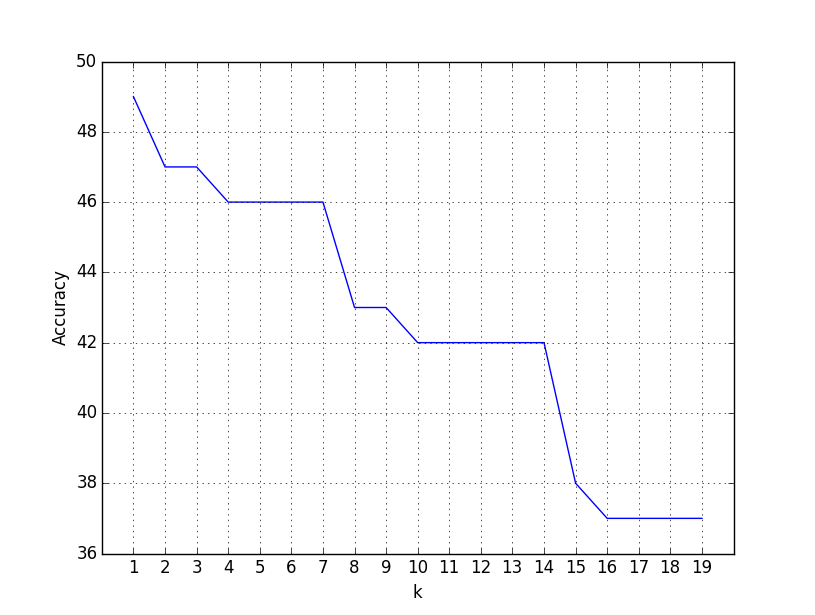
\includegraphics[width=.9\textwidth]{knn_kd_iris}
\caption{Accuracy of the $k$-nearest neighbors classifier using a $kd$-tree for $1 \leq k \leq 19$ on the Iris data set.}
\label{knn_iris}
\end{figure}

The $k$-nearest neighbors classifier achieved a maximum classification rate of $96.08\%$ accuracy for $k=1$.

\subsubsection{UCI Wine Data Set}
\begin{figure}[H]
\centering
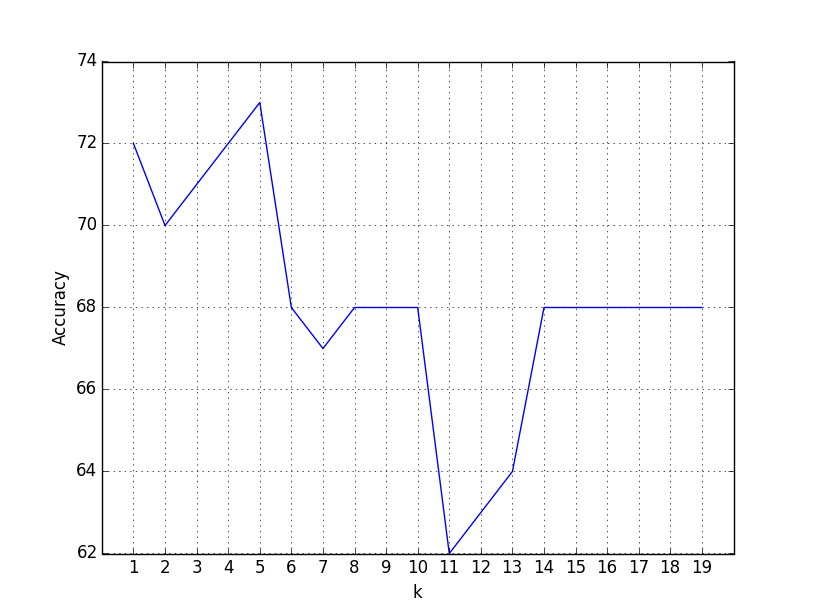
\includegraphics[width=.9\textwidth]{knn_kd_wine}
\caption{The accuracy of the $k$-nearest neighbors classifier using a $kd$-tree for $1 \leq k \leq 19$ on the UCI wine data set.}
\label{knn_wine}
\end{figure}

Here, the $k$-nearest neighbors classifier achieved a maximum classification rate of $82.02\%$ accuracy for $k=5$.

%~~~~~~~~~~~~~~~~~~~~~~~~~~~~~~~~
\subsubsection{Handwritten Digits Data Set}


%%%%%%%%%%%%%%%%%%%%%%%%%%%%%%%%%%%%%%%%%%%%%%%%%%%%%%%%%%%%%%%%%%%%%%%%%%%%%%%%%%%
\section{Analysis}
\todo{You need to compare different methods in terms of classification performance and required time for classification, and give justifications for your observed empirical results.}

%%%%%%%%%%%%%%%%%%%%%%%%%%%%%%%%%%%%%%%%%%%%%%%%%%%%%%%%%%%%%%%%%%%%%%%%%%%%%%%%%%%

\section{Extra Credit}
\todo{Please state clearly in your report if you have implemented any of the following extra
credit options.}

%~~~~~~~~~~~~~~~~~~~~~~~~~~~~~~~~
\subsection{Recognition of my handwritten digits}
\todo{Apply the best classifier you have for hand written digit recognition on a test set consisting of your own written digits (you need to create the dataset). Document the classification performance, what you have done to improve the performance, and any additional issues you have handled.}

%%%%%%%%%%%%%%%%%%%%%%%%%%%%%%%%%%%%%%%%%%%%%%%%%%%%%%%%%%%%%%%%%%%%%%%%%%%%%%%%%%%

\begin{thebibliography}{9}

\bibitem{sp}
    Jones E, Oliphant E, Peterson P, \emph{et al.}
    {\bf SciPy: Open Source Scientific Tools for Python}, 2001-,
    \url{http://www.scipy.org/} [Online; accessed 2015-10-24].

\end{thebibliography}

%%%%%%%%%%%%%%%%%%%%%%%%%%%%%%%%%%%%%%%%%%%%%%%%%%%%%%%%%%%%%%%%%%%%%%%%%%%%%%%%%%%

\end{document}